\documentclass[9pt,table]{beamer} % options fleqn

\usepackage{/home/paul/Workspace/build/macros}


\usetheme[titleformat frame = smallcaps]{metropolis}
%\usepackage{FiraSans}
\usepackage{FiraMono}

\metroset{sectionpage=none}

%\usepackage[T1]{fontenc}


%\setbeamersize{text margin left=5mm,text margin right=5mm} 
%\setbeamersize{text margin left=9mm,text margin right=3mm} 

\setbeamertemplate{section in toc}[sections numbered]

% algorithms
\usepackage[ruled,linesnumbered]{algorithm2e}
\SetKwInput{KwInput}{Input}
\SetKwInput{KwOutput}{Output}

% typography
\usepackage{soul}

\usepackage{caption}

\usepackage{varwidth}

\usepackage{dsfont}

% drawings
\usepackage{tikz}
\usetikzlibrary{shapes,shapes.misc,shapes.geometric}
\usetikzlibrary{positioning,fit,backgrounds}
\usetikzlibrary{trees,matrix}
\usetikzlibrary{decorations.pathreplacing,calligraphy}
%
\tikzset{cross/.style={cross out, draw=red, minimum size=3pt, line width=0.25mm, inner sep=0pt, outer sep=0pt}, cross/.default={1pt}}
%
\usepackage[skins,theorems]{tcolorbox}
\tcbset{highlight math style={colback=mLightBrown!20,colframe=black!2,sharp corners},bottom=2pt,top=2pt}
\tcbset{left skip={-.01\linewidth}, colback=mLightBrown!20,colframe=black!2,sharp corners,left=0pt,right=0pt}
%
\newcommand{\point}[1]{\textbf{\textcolor{mDarkTeal}{#1}}\quad}
%
%\definecolor{cobalt}{HTML}{0047AB}
\definecolor{aqua}{HTML}{00FFFF}
\newcommand{\kw}[1]{\textbf{\alert{#1}}}
\newcommand{\invsible}[1]{\textcolor{black!2}{#1}}
%
\definecolor{myteal}{rgb}{0.21, 0.46, 0.53}

\usepackage[position=bottom]{subfig}

\usepackage{tabularx}
\usepackage{booktabs}% http://ctan.org/pkg/booktabs
\newcommand{\tabitem}{\llap{\tiny$\blacksquare$}~~}

% handling lists
\usepackage{enumitem}

\usepackage{multimedia}

% tcolorbox
\usepackage[skins,theorems]{tcolorbox}
\tcbset{highlight math style={colback=mLightBrown!20,colframe=black!2,sharp corners},bottom=2pt,top=2pt}
\tcbset{left skip={-.01\linewidth}, colback=mLightBrown!20,colframe=black!2,sharp corners,left=0pt,right=0pt}


% references
\usepackage[backend=biber,style=authoryear]{biblatex}
%\usepackage[backend=biber,style=alphabetic]{biblatex}
\bibliography{/home/paul/Workspace/build/biblio}
\usepackage{bibentry}
\newcommand{\mycite}[2]{\footnotetext[#1]{\emph{\tiny{\citeauthor{#2},\,\citeyear{#2},}}\,\tiny{\citefield{#2}{title}}}}

%\renewcommand{\cite}[1]{\textcolor{myteal}{[\citeauthor{#1},\,\citeyear{#1}]}}%
%\newcommand{\mycite}[1]{\textcolor{myteal}{\cite{#1}}}%
\AtBeginEnvironment{frame}{\setcounter{footnote}{0}}

\usepackage{hyperref}


\graphicspath{{figs/}{examples/}{/home/paul/Workspace/data/standard_test_images}}




% add a sommaire
%\makeatletter
%\setbeamertemplate{headline}{%
%  \begin{beamercolorbox}[colsep=1.5pt]{upper separation line head}
%  \end{beamercolorbox}
%  \begin{beamercolorbox}{section in head/foot}
%    \vskip2pt\insertnavigation{\paperwidth}\vskip2pt
%  \end{beamercolorbox}%
%  \begin{beamercolorbox}[colsep=1.5pt]{lower separation line head}
%  \end{beamercolorbox}
%}
%\makeatother

\setbeamertemplate{theorem begin}
{%
  \inserttheoremheadfont% \bfseries
  \inserttheoremname \inserttheoremnumber
  \ifx\inserttheoremaddition\@empty\else\ (\inserttheoremaddition)\fi%
  \inserttheorempunctuation
  \normalfont
}
\setbeamertemplate{theorem end}{%
  % empty
}
\makeatother

\setbeamercolor{section in head/foot}{fg=normal text.bg, bg=structure.fg}



\title{Optimisation Numérique et Sciences des Données}
\subtitle{Optimisation numérique -- Introduction}
\author{Paul Catala (CRAN) \hfill M2 ISC 925}
%\date{Postdoctorant à l'université d'Osnabrück, Allemagne}
\date{paul.catala@gmail.com \hfill Septembre 2024 \\ \\ Cours élaboré par Julien Flamant}

%\usepackage{uoslogo}
%\titlegraphic{\uoslogored{4cm}}



\begin{document}
\maketitle


\section{Un premier exemple introductif}

\begin{frame}
\frametitle{Programme du cours}
\tableofcontents[currentsection]
\end{frame}


\begin{frame}
\frametitle{Exemple Introductif}

\begin{columns}

% ******************* c1

\begin{column}{0.68\textwidth}

\begin{itemize}[label=\tiny$\blacksquare$]
	\item Un fabricant de boîtes de conserve souhaite \alert{optimiser} sa consommation de matière première
	
	\item Seule \alert{contrainte} du problème: leur volume $V = V_0$ est fixé
\end{itemize}



\end{column}

% ******************* c2

\begin{column}{0.3\textwidth}
\begin{tikzpicture}
\node[cylinder, draw,
		shape border rotate = 90,
		cylinder uses custom fill, 
		cylinder body fill = mLightBrown!40, 
		cylinder end fill = mLightBrown!20,
		minimum width = 3cm,
		minimum height = 4cm,
		aspect = 6] (cylindre) {};
		
\draw[|-|,thick,teal] ([xshift=-.3cm,yshift=.3cm]cylindre.north west) -- ([xshift=-.55cm,yshift=.2cm]cylindre.south west) node[midway,fill=black!2]{h};

\draw[{Circle[teal]}-,thick,teal] ([yshift=-.5cm]cylindre.north) -- ([xshift=0.95cm,yshift=-.15cm]cylindre.north) node[midway,below] {r};
\end{tikzpicture}
\end{column}

% ******************* end

\end{columns}



Formulation du problème d'optimisation de forme

quantité de matière première = aire du cylindre $\times$ épaisseur (constante)

comment \alert{minimiser} l'aire A d'un cylindre droit de volume V fixé?

\end{frame}


\begin{frame}
\frametitle{Formulation Mathématique}

\begin{itemize}[label=\tiny$\blacksquare$]
	\item Expression de l'aire $A$ (\alert{fonction objectif})
		\eq{
			A(r,h) \eqdef 2\pi r h + 2\pi r^2
		}
	
	
	
	\item Les dimensions $r$ et $h$ sont les \alert{variables} du problème \\ Elles doivent être positives (\alert{contraintes})
	\eq{
		r \geq 0, \quad h \geq 0
	}
	
	
	
	\item La condition de volume constant est aussi une \alert{contrainte}: 
	\eq{
		V(r,h) = \pi h r^2 = V_0
	}



	\item Finalement, le \alert{problème d'optimisation sous contraintes} s'écrit
	\eq{
		\text{minimiser} \quad A(r,h) \quad \text{sous les contraintes} \quad
		\left\{\begin{aligned}
			& r \geq 0, h \geq 0 \\
			& \pi h r^2 = V_0
		\end{aligned}\right.
	}
\end{itemize}

\end{frame}







\begin{frame}
\frametitle{Simplification du Problème}

\begin{itemize}[label=\tiny$\blacksquare$]
	\item $h$ et $r$ sont liés par la contrainte de volume fixe
	\eq{
		h(r) = \frac{V_0}{\pi r^2}
	}
	Cette expression satisfait bien la contrainte $h \geq 0$.
	\item En remplaçant dans $A(h,r)$, on obtient
	\eq{
		A(h,r) = 2\pi r h + 2\pi r^2 = \frac{2\pi V_0}{r} + 2\pi r^2 \defeq \tilde{A}(r)
	}
	La contrainte de volume est prise en compte directement dans la nouvelle fonction objectif $\tilde{A}(r)$.
	
	\item Le problème d'optimisation s'écrit de manière équivalente
	\eq{
		\text{minimiser} \quad \tilde{A}(r) \quad \text{sous la contrainte} \quad r \geq 0
	}
\end{itemize}
\end{frame}




\begin{frame}
\frametitle{Visualisation}

\begin{figure}
	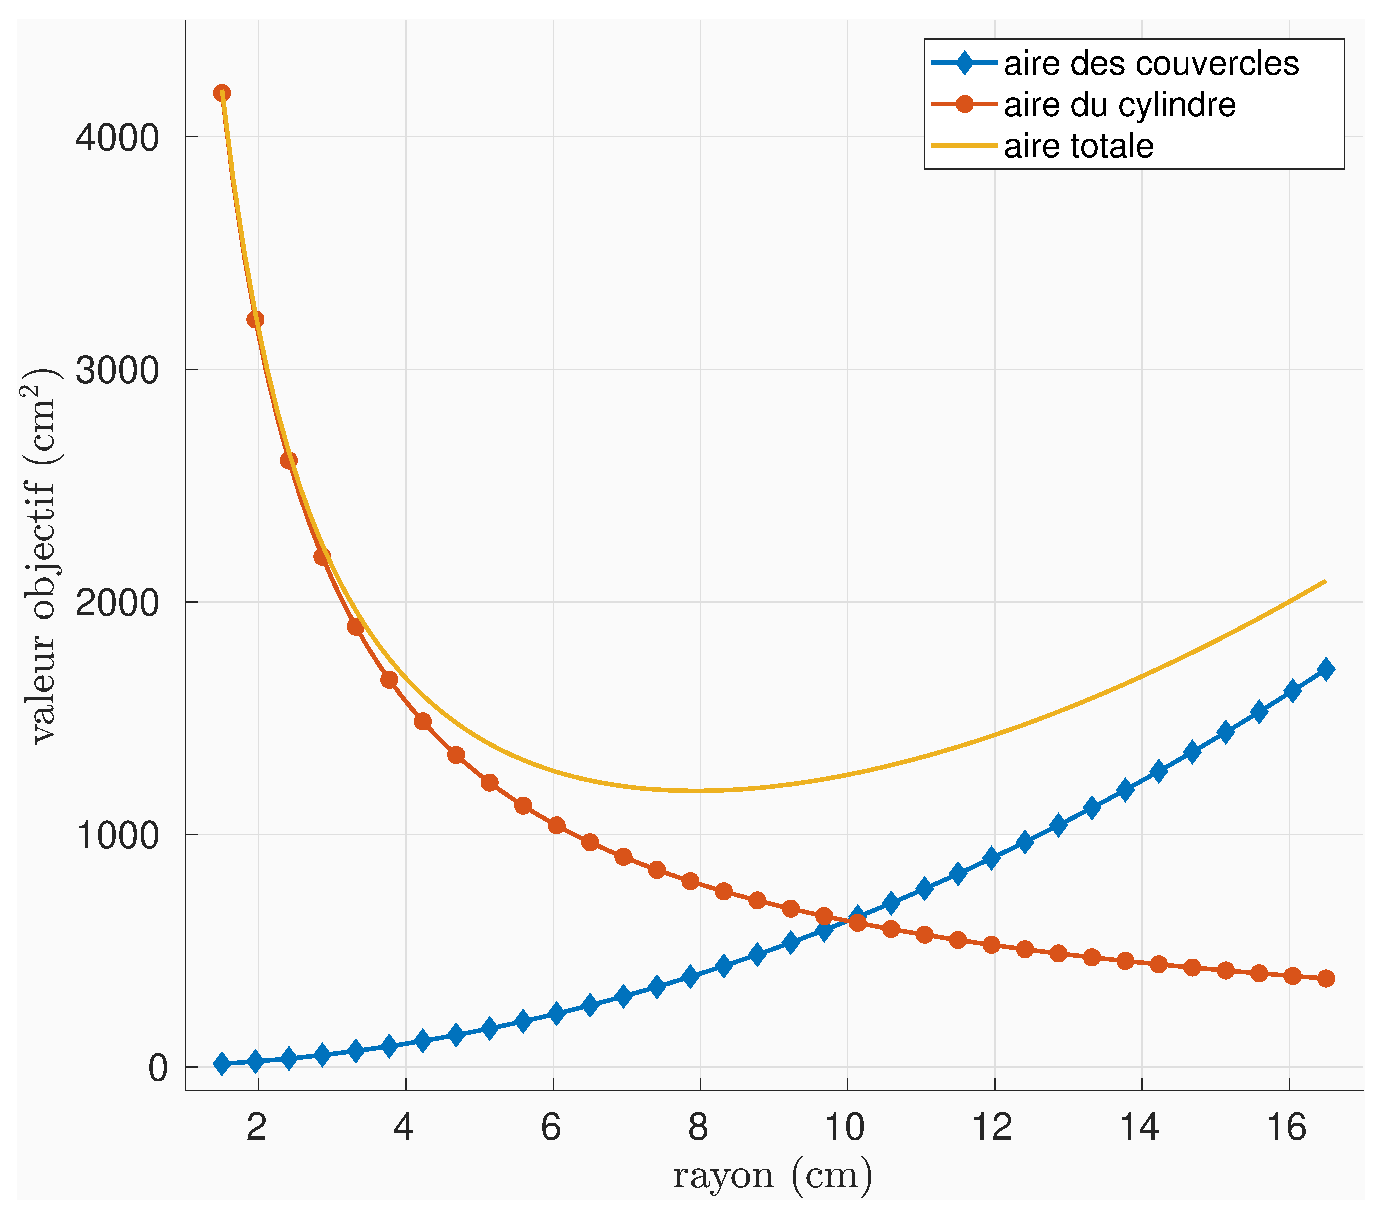
\includegraphics[width=0.8\textwidth]{exemple-introductif}
\end{figure}
\end{frame}



\section{Exemples}


\begin{frame}
\frametitle{Programme du cours}
\tableofcontents[currentsection]
\end{frame}


\begin{frame}
\frametitle{Problème de Transport}


\begin{itemize}[label=\tiny$\blacksquare$]
	\item Soient $N$ entrepôts, $M$ magasins. Chaque entrepôt $i$ dispose de $a_i$ unités d'un certain produit, chaque magasin $j$ a une demande $b_j$ de ce produit.
	
	\item Transporter une unité de l'entrepôt $i$ au magasin $j$ coûte $c_{ij}$
\end{itemize}

%\begin{columns}

% ************ c1

%\begin{column}{0.4\textwidth}

\begin{center}
\begin{tikzpicture}
\node[circle, draw, color=teal, scale=0.75] at (1.7156, 1.2662) (m1) {15};
\node[circle, draw, color=teal, scale=0.7] at (1.0078, -1.8684) (m2) {14};
\node[circle, draw, color=teal, scale=0.45] at (-0.3210, -0.8459) (m3) {9};
\node[circle, draw, color=teal, scale=1] at (-1.7278, -0.8010) (m4) {62};

\node[rectangle, fill=mLightBrown!80, draw, scale=0.4] at (-2.4318, 1.2639) (e1) {8};
\node[rectangle, fill=mLightBrown!80, draw, scale=1.5] at (-1.6777, -2.482) (e2) {30};
\node[rectangle, fill=mLightBrown!80, draw, scale=0.45] at (-0.9264, -2.4437) (e3) {9};
\node[rectangle, fill=mLightBrown!80, draw, scale=1.8] at (-0.8234, 0.7724) (e4) {36};
\node[rectangle, fill=mLightBrown!80, draw, scale=0.85] at (-0.4081, -1.8576) (e5) {17};

\pause

\draw[-latex] (e1) -- (m4) node[midway,fill=black!2] {8};
\draw[-latex] (e2) -- (m4) node[midway,fill=black!2] {30};
\draw[-latex] (e3) -- (m4) node[midway,fill=black!2] {9};
\draw[-latex] (e4) -- (m1) node[midway,fill=black!2] {15};
\draw[-latex] (e4) -- (m3) node[midway,fill=black!2] {6};
\draw[-latex] (e4) -- (m4) node[midway,fill=black!2] {15};
\draw[-latex] (e5) -- (m2) node[midway,fill=black!2] {14};
\draw[-latex] (e5) -- (m3) node[midway,fill=black!2] {3};


\end{tikzpicture}

%\end{column}

% ***************** c2

%\begin{column}{0.5\textwidth}

%\end{column}

% *****************

%\end{columns}

\onslide<2>{
Objectif: minimiser le coût total de transport

Variables: les $N \times M$ couplages possibles $T_{ij}$
}

\end{center}
\end{frame}






\begin{frame}
\frametitle{Entraînement d'un Réseau de Neurones}

\newlength{\spacing}
\setlength{\spacing}{1.5cm}

\vspace{-1cm}

\centering

\begin{tikzpicture}[every node/.style={circle,minimum width = .5cm}]

% first layer
\node[draw] (n10) at (0,0) {$x_1$};
\node[draw,below=5pt of n10] (n11) {$x_2$};
\node[draw,below=5pt of n11] (n12) {$x_3$};
\node[draw,below=5pt of n12] (n13) {$x_4$};


% second layer
\node[draw,above right = 0.77cm and \spacing of n10] (n20) {};
\node[draw,below=5pt of n20] (n21) {};
\node[draw,below=5pt of n21] (n22) {};
\node[draw,below=5pt of n22] (n23) {};
\node[draw,below=5pt of n23] (n24) {};
\node[draw,below=5pt of n24] (n25) {};
\node[draw,below=5pt of n25] (n26) {};
\node[draw,below=5pt of n26] (n27) {};

% connections
\draw[] (n10) -- (n20);
\draw[] (n10) -- (n21);
\draw[] (n10) -- (n22);
\draw[] (n10) -- (n23);
\draw[] (n10) -- (n24);
\draw[] (n10) -- (n25);
\draw[] (n10) -- (n26);
\draw[] (n10) -- (n27);
%
\draw[] (n11) -- (n20);
\draw[] (n11) -- (n21);
\draw[] (n11) -- (n22);
\draw[] (n11) -- (n23);
\draw[] (n11) -- (n24);
\draw[] (n11) -- (n25);
\draw[] (n11) -- (n26);
\draw[] (n11) -- (n27);
%
\draw[] (n12) -- (n20);
\draw[] (n12) -- (n21);
\draw[] (n12) -- (n22);
\draw[] (n12) -- (n23);
\draw[] (n12) -- (n24);
\draw[] (n12) -- (n25);
\draw[] (n12) -- (n26);
\draw[] (n12) -- (n27);
%
\draw[] (n13) -- (n20);
\draw[] (n13) -- (n21);
\draw[] (n13) -- (n22);
\draw[] (n13) -- (n23);
\draw[] (n13) -- (n24);
\draw[] (n13) -- (n25);
\draw[] (n13) -- (n26);
\draw[] (n13) -- (n27);


% third layer
\node[draw,below right = 0.3cm and \spacing of n20] (n30) {};
\node[draw,below=5pt of n30] (n31) {};
\node[draw,below=5pt of n31] (n32) {};
\node[draw,below=5pt of n32] (n33) {};
\node[draw,below=5pt of n33] (n34) {};
\node[draw,below=5pt of n34] (n35) {};

% connections
\draw[] (n20) -- (n30);
\draw[] (n20) -- (n31);
\draw[] (n20) -- (n32);
\draw[] (n20) -- (n33);
\draw[] (n20) -- (n34);
\draw[] (n20) -- (n35);
%
\draw[] (n21) -- (n30);
\draw[] (n21) -- (n31);
\draw[] (n21) -- (n32);
\draw[] (n21) -- (n33);
\draw[] (n21) -- (n34);
\draw[] (n21) -- (n35);
%
\draw[] (n22) -- (n30);
\draw[] (n22) -- (n31);
\draw[] (n22) -- (n32);
\draw[] (n22) -- (n33);
\draw[] (n22) -- (n34);
\draw[] (n22) -- (n35);
%
\draw[] (n23) -- (n30);
\draw[] (n23) -- (n31);
\draw[] (n23) -- (n32);
\draw[] (n23) -- (n33);
\draw[] (n23) -- (n34);
\draw[] (n23) -- (n35);
%
\draw[] (n24) -- (n30);
\draw[] (n24) -- (n31);
\draw[] (n24) -- (n32);
\draw[] (n24) -- (n33);
\draw[] (n24) -- (n34);
\draw[] (n24) -- (n35);
%
\draw[] (n25) -- (n30);
\draw[] (n25) -- (n31);
\draw[] (n25) -- (n32);
\draw[] (n25) -- (n33);
\draw[] (n25) -- (n34);
\draw[] (n25) -- (n35);
%
\draw[] (n26) -- (n30);
\draw[] (n26) -- (n31);
\draw[] (n26) -- (n32);
\draw[] (n26) -- (n33);
\draw[] (n26) -- (n34);
\draw[] (n26) -- (n35);
%

\draw[] (n27) -- (n30);
\draw[] (n27) -- (n31);
\draw[] (n27) -- (n32);
\draw[] (n27) -- (n33);
\draw[] (n27) -- (n34);
\draw[] (n27) -- (n35);


% fourth layer
\node[draw,above right = 0.3cm and \spacing of n30] (n40) {};
\node[draw,below=5pt of n40] (n41) {};
\node[draw,below=5pt of n41] (n42) {};
\node[draw,below=5pt of n42] (n43) {};
\node[draw,below=5pt of n43] (n44) {};
\node[draw,below=5pt of n44] (n45) {};
\node[draw,below=5pt of n45] (n46) {};
\node[draw,below=5pt of n46] (n47) {};


% connections
\draw[] (n30) -- (n40);
\draw[] (n30) -- (n41);
\draw[] (n30) -- (n42);
\draw[] (n30) -- (n43);
\draw[] (n30) -- (n44);
\draw[] (n30) -- (n45);
\draw[] (n30) -- (n46);
\draw[] (n30) -- (n47);
%
\draw[] (n31) -- (n40);
\draw[] (n31) -- (n41);
\draw[] (n31) -- (n42);
\draw[] (n31) -- (n43);
\draw[] (n31) -- (n44);
\draw[] (n31) -- (n45);
\draw[] (n31) -- (n47);
%
\draw[] (n32) -- (n40);
\draw[] (n32) -- (n41);
\draw[] (n32) -- (n42);
\draw[] (n32) -- (n43);
\draw[] (n32) -- (n44);
\draw[] (n32) -- (n45);
\draw[] (n32) -- (n46);
\draw[] (n32) -- (n47);
%
\draw[] (n33) -- (n40);
\draw[] (n33) -- (n41);
\draw[] (n33) -- (n42);
\draw[] (n33) -- (n43);
\draw[] (n33) -- (n44);
\draw[] (n33) -- (n45);
\draw[] (n33) -- (n46);
\draw[] (n33) -- (n47);
%
\draw[] (n34) -- (n40);
\draw[] (n34) -- (n41);
\draw[] (n34) -- (n42);
\draw[] (n34) -- (n43);
\draw[] (n34) -- (n44);
\draw[] (n34) -- (n45);
\draw[] (n34) -- (n46);
\draw[] (n34) -- (n47);
%
\draw[] (n35) -- (n40);
\draw[] (n35) -- (n41);
\draw[] (n35) -- (n42);
\draw[] (n35) -- (n43);
\draw[] (n35) -- (n44);
\draw[] (n35) -- (n45);
\draw[] (n35) -- (n46);
\draw[] (n35) -- (n47);
%

% output layer
\node[draw,below right = 2cm and \spacing of n40] (n50) {$y$};
%\node[below=5pt of n50] (n51) {$y_2$};
%\node[below=5pt of n51] (n52) {$y_3$};


% connections
\draw[] (n40) -- (n50);
%\draw[] (n40) -- (n51);
%\draw[] (n40) -- (n52);
%
\draw[] (n41) -- (n50);
%\draw[] (n41) -- (n51);
%\draw[] (n41) -- (n52);
%
\draw[] (n42) -- (n50);
%\draw[] (n42) -- (n51);
%\draw[] (n42) -- (n52);
%
\draw[] (n43) -- (n50);
%\draw[] (n43) -- (n51);
%\draw[] (n43) -- (n52);
%
\draw[] (n44) -- (n50);
%\draw[] (n44) -- (n51);
%\draw[] (n44) -- (n52);
%
\draw[] (n45) -- (n50);
%\draw[] (n45) -- (n51);
%\draw[] (n45) -- (n52);
%
\draw[] (n46) -- (n50);
%\draw[] (n46) -- (n51);
%\draw[] (n46) -- (n52);
%
\draw[] (n47) -- (n50);
%\draw[] (n47) -- (n51);
%\draw[] (n47) -- (n52);


\begin{scope}[on background layer]
\node [rectangle, fill=mLightBrown!20, minimum height = 5.6cm, fit={(n10) (n11) (n12) (n13) }, label={[label distance = -23pt]\color{mLightBrown}Couche d'entrée}] (layer-1) {};

\node [rectangle, fill=teal!20, minimum height = 5.6cm, fit={(n20) (n21) (n22) (n23) (n24) (n25) (n26) (n27)}] (layer-2) {};

\node [rectangle, fill=teal!20, minimum height = 5.6cm, fit={(n30) (n31) (n32) (n33) (n34) (n35) }, label={[label distance = -25pt]\color{teal}Couches latentes}] (layer-3) {};

\node [rectangle, fill=teal!20, minimum height = 5.6cm, fit={(n40) (n41) (n42) (n43) (n44) (n45) (n46) (n47)}] (layer-4) {};

\node [rectangle, fill=purple!20, minimum height = 5.6cm, fit={(n50)}, label={[label distance = -25pt]\color{purple}Couche de sortie}] (layer-5) {};
\end{scope}

\draw[-latex,thick] ([yshift=-.3cm]layer-1.south west) -- ([yshift=-.3cm]layer-5.south east) node[rectangle,midway,fill=black!2] {$y = f_\theta(x)$};

\end{tikzpicture}

Objectif: minimiser l'erreur $\sum_j \ell(f_\theta(x^{(j)}),y^{(j)})$ sur des données $(x^{(j)},y^{(j)})$

Variables: $\sim 10^6$ à $10^9$ paramètres $\theta$

\end{frame}



\section{Terminologie}


\begin{frame}
\frametitle{Programme du cours}
\tableofcontents[currentsection]
\end{frame}




%\begin{frame}
%\frametitle{Qu'est-ce qu'un problème d'optimisation?}
%
%Soient $n \in \NN$, \quad $f : \RR^n \to \RR$, \quad $X \subset \RR^n$,
%
%\eq{
%	\min \quad f(x) \qscq x \in X
%}
%
%\begin{itemize}[label=\tiny$\blacksquare$]
%	\item $f$ est la \alert{fonction objectif}, ou \alert{fonction coût}, ou \alert{critère}
%	
%	\item $X$ est l'\alert{ensemble des contraintes}
%\end{itemize}
%\end{frame}



\begin{frame}
\frametitle{Terminologie}

Soient $f, c_1, \ldots, c_m$ des fonctions

\eq{
	\min_{x \in \XX^n} \quad f(x) \qscq \left\{
		\begin{aligned}
			&c_i(x) = 0 \quad i \in \Ee \\
			&c_i(x) \leq 0 \quad i \in \Ii
		\end{aligned}
		\right.
}

\begin{itemize}[label=\tiny$\blacksquare$]
	\item $f:\XX^N \to \RR$ est la \alert{fonction coût}, ou \alert{fonction objectif}, ou \alert{critère}
	\item $c_1,\ldots,c_m : \XX^N \to \RR$ sont les \alert{fonctions de contraintes} du problème
	\begin{itemize}
		\item $\Ee$ (éventuellement $\emptyset$) numérote les \alert{contraintes d'égalité}
		\item $\Ii$ (éventuellement $\emptyset$) numérote les \alert{contraintes d'inégalité}
	\end{itemize}
	\item $\Dd \eqdef \enscond{x\in \XX^N}{c_i(x) = 0\; \forall i \in \Ee, \quad c_i(x) \leq 0\; \forall i \in \Ii}$ est le \alert{domaine d'optimisation}
\end{itemize}

\end{frame}



\begin{frame}
\frametitle{Nomenclature}

\begin{tikzpicture}
\node[rectangle,fill=mLightBrown!40] at (0,0) (optim-num) {Optimisation numérique};
\node[right = 0.5em of optim-num] (dots) {:};
\node[rectangle,right=0.5em of dots] (optim-d) {Optimisation discrète};
\node[right = 0.5em of optim-d] (vs) {vs};
\node[rectangle,fill=mLightBrown!30,right=0.5em of vs] (optim-c) {Optimisation continue};

\node[below=0.5em of optim-num] {$\XX \subset \RR$};
\node[below=0.5em of optim-d] {$\XX$ fini ou discret};
\node[below=0.5em of optim-c] {$\XX = \RR$};

\node[draw,rectangle,below = 3em of optim-d] (optim-cvx) {Programmation convexe};
\node[draw,rectangle,right = 3em of optim-cvx] (optim-l) {Programmation linéaire};

\node[draw,rectangle,right = 3em of optim-l] (optim-nl) {Programmation non-linéaire};
\end{tikzpicture}

\end{frame}






%\bibliographystyle{apalike}
%\printbibliography
%\bibliography{/export/home/pcatala/Workspace/build/biblio}

\end{document}
